\documentclass[UTF8]{ctexart}
\usepackage[left=2cm,right=2cm,top=2cm]{geometry}
\usepackage{amsmath}
\usepackage{enumitem}
\usepackage{float}
\usepackage{threeparttable}
\usepackage{caption}
\usepackage{multirow}
\usepackage{graphicx}
\usepackage{listings}
\usepackage{color}
\definecolor{dkgreen}{rgb}{0,0.6,0}
\definecolor{gray}{rgb}{0.5,0.5,0.5}
\definecolor{mauve}{rgb}{0.58,0,0.82}
\lstset{frame=tb,
  language=C++,
  aboveskip=3mm,
  belowskip=3mm,
  showstringspaces=false,
  columns=flexible,
  basicstyle={\small\ttfamily},
  numbers=left,%设置行号位置none不显示行号
  %numberstyle=\tiny\courier, %设置行号大小
  numberstyle=\tiny\color{gray},
  keywordstyle=\color{blue},
  commentstyle=\color{dkgreen},
  stringstyle=\color{mauve},
  breaklines=true,
  breakatwhitespace=true,
  escapeinside=`,%逃逸字符(1左面的键),用于显示中文例如在代码中`中文...`
  tabsize=4,
  extendedchars=false %解决代码跨页时,章节标题,页眉等汉字不显示的问题
}

\setlength\lineskiplimit{5.25bp}
\setlength\lineskip{5.25bp}

\title{计算方法第六次编程作业报告}
\author{崔士强 PB22151743}
\date{\today}

\bibliographystyle{plain}

\begin{document}

\maketitle

\section{问题描述}
本程序实现对一个函数(以及添加了随机噪声的形式)的快速Fourier变换及逆变换。

\section{问题分析}
首先对函数进行采样,采样点的个数应当是$2$的$n$次幂. 采样后的向量$\mathbf{f}$作为FFT算法的输入,得到g,若想重建
函数,可以将变换后的向量输入IFFT算法.

\section{实验结果}
\subsection{结果展示}
\begin{enumerate}
  \item $f_1, n=8$
\begin{figure}[H]
    \centering
    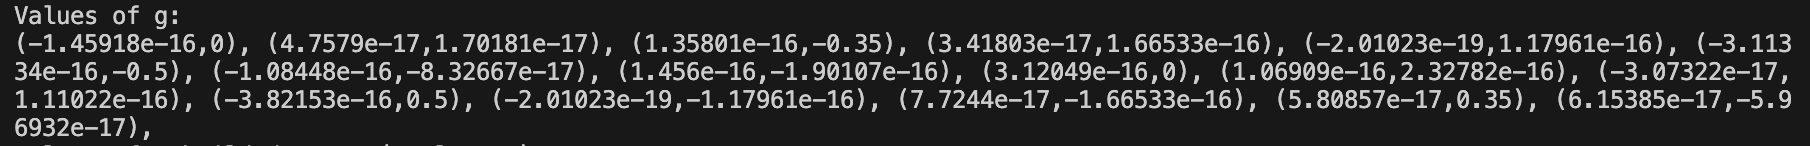
\includegraphics[scale=0.5]{g_1.png}
    \caption{FFT结果}
\end{figure}
可以看到$\mathbf{g}$的大部分分量都接近0
\begin{figure}[H]
  \centering
  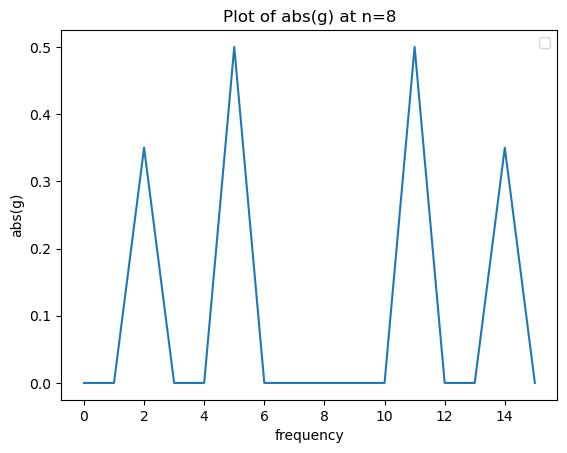
\includegraphics[scale=0.5]{g_abs_1.png}
  \caption{$\mathbf{g}$的每个分量模长}
\end{figure}
\begin{figure}[H]
  \centering
  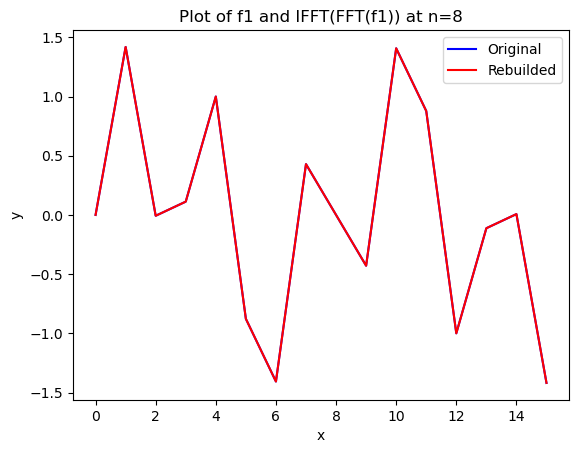
\includegraphics[scale=0.5]{res_1.png}
  \caption{原数据与重建结果}
\end{figure}
由于采样点较少,获得的折线图较为粗糙地反映了函数的情况. 重建结果与原本的采样结果基本一致.

  \item $f_1, n=128$
\begin{figure}[H]
    \centering
    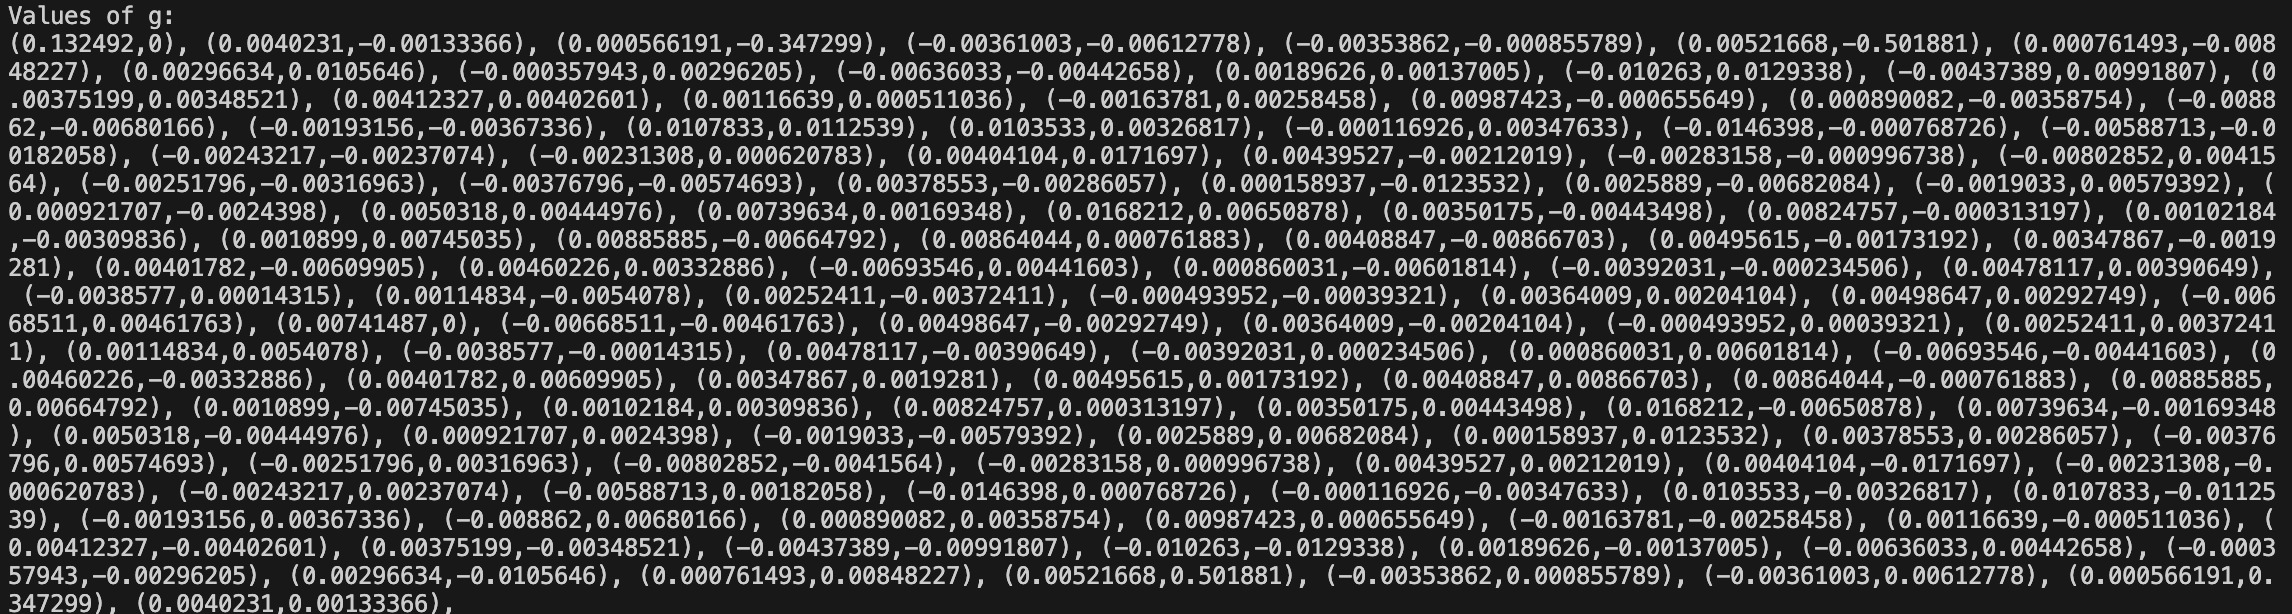
\includegraphics[scale=0.3]{g_2.png}
    \caption{FFT结果}
\end{figure}
可以看到$\mathbf{g}$的大部分分量同样都接近0,非零分量集中在频率两端
\begin{figure}[H]
  \centering
  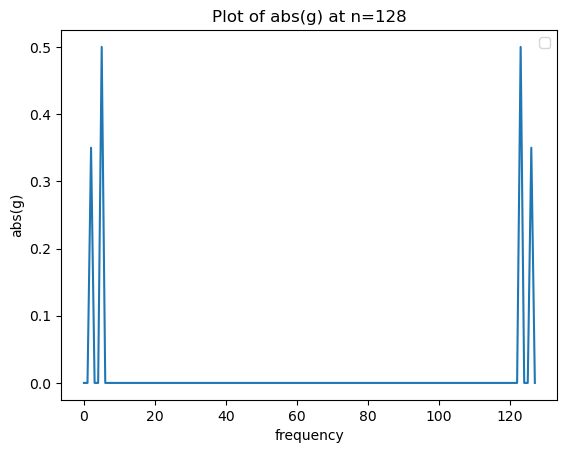
\includegraphics[scale=0.5]{g_abs_2.png}
  \caption{$\mathbf{g}$的每个分量模长}
\end{figure}
\begin{figure}[H]
  \centering
  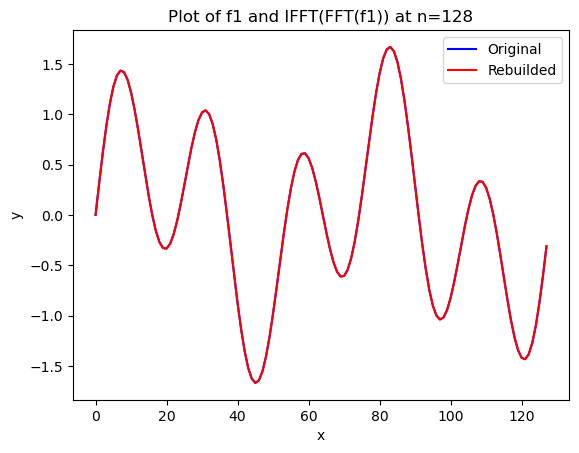
\includegraphics[scale=0.5]{res_2.png}
  \caption{原数据与重建结果}
\end{figure}
采样点较多时,采样结果基本还原函数的情况. 重建结果与原本的采样结果基本一致.

  \item $f_2, n=128$
\begin{figure}[H]
    \centering
    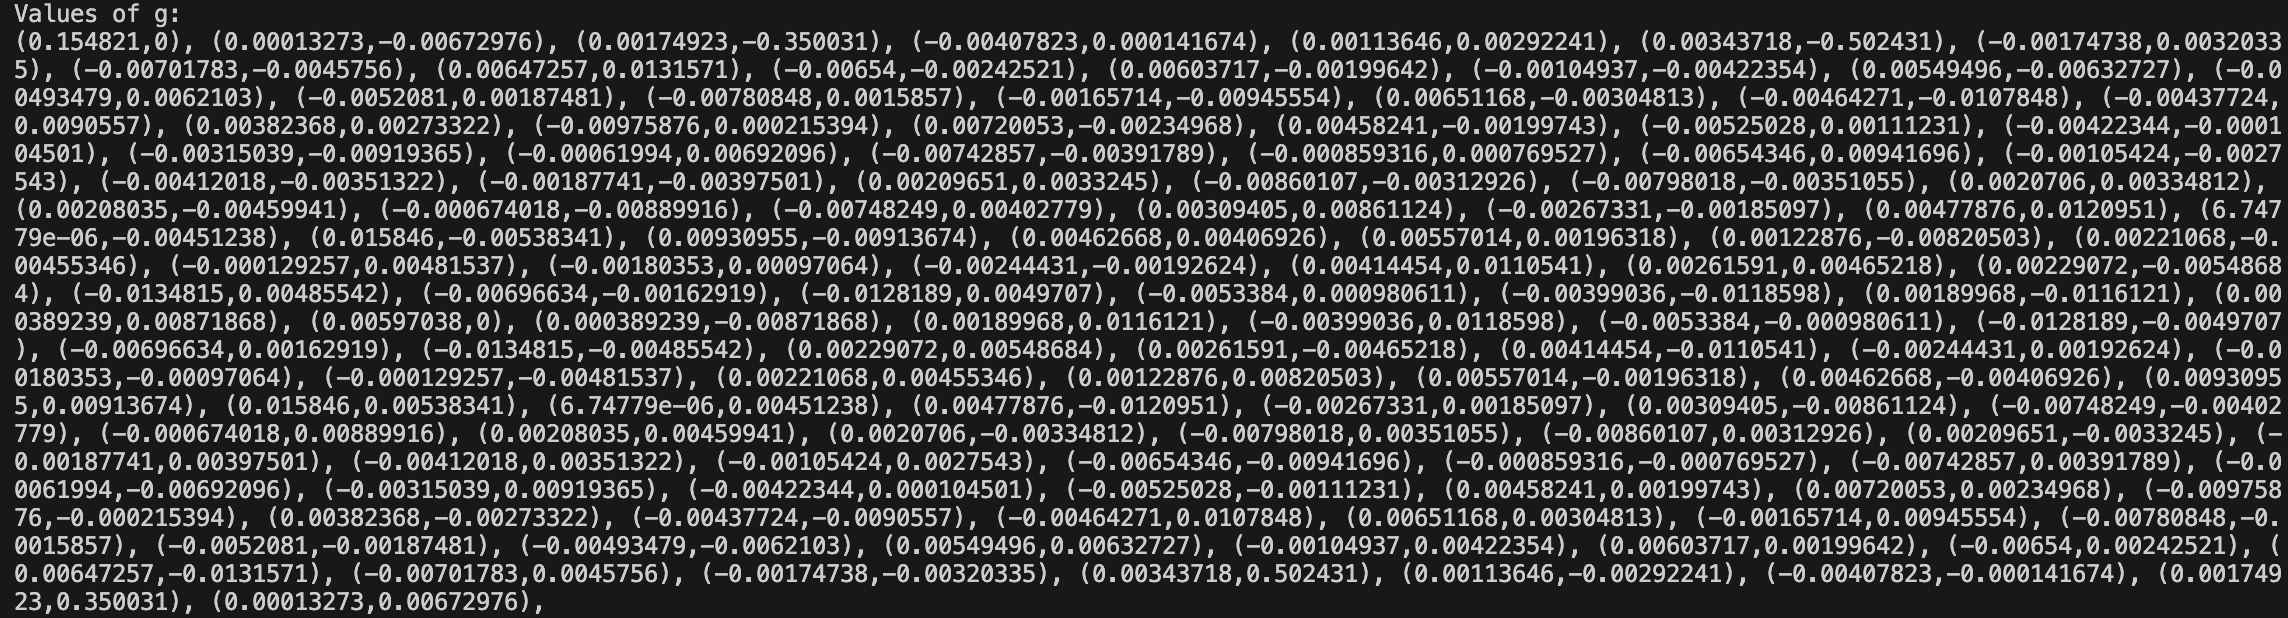
\includegraphics[scale=0.3]{g_3.png}
    \caption{FFT结果}
\end{figure}
\begin{figure}[H]
  \centering
  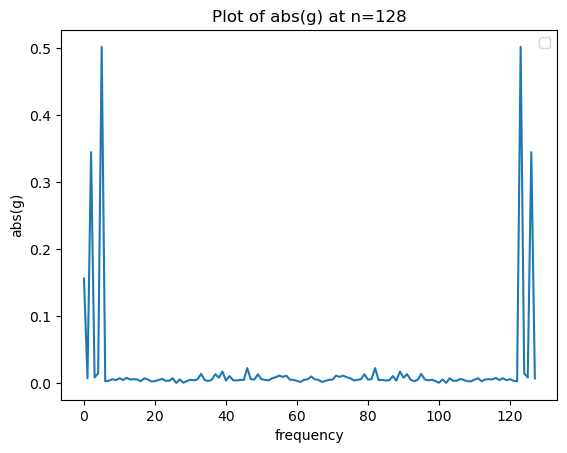
\includegraphics[scale=0.5]{g_abs_3.png}
  \caption{$\mathbf{g}$的每个分量模长}
\end{figure}
添加噪声后在中间位置的频率也出现了一些非零分量
\begin{figure}[H]
  \centering
  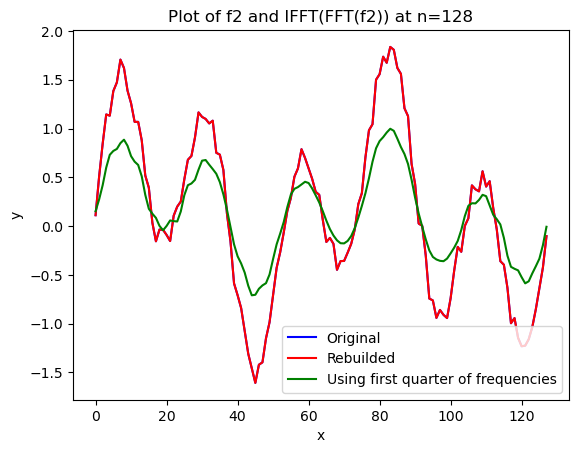
\includegraphics[scale=0.5]{res_3.png}
  \caption{原数据与重建结果}
\end{figure}
采样点较多时,采样结果基本还原函数的情况. 重建结果与原本的采样结果基本一致.
\end{enumerate}

\subsection{结果分析}
\begin{enumerate}
  \item 从运行结果可以看到,$n$较大时采样结果更能完整反映函数情况,$\mathbf{g}$的非零分量明显集中在两端
  \item 去掉高频系数进行重建后,所的结果的方差明显变小,噪声导致的不光滑有所缓解.
\end{enumerate}


\bibliography{math}

\end{document}
\iffalse
\begin{figure}[h]
    \centering
    \includegraphics[scale=0.5]{name.png}
    \caption{name}
\end{figure}
\fi
